\documentclass[border=0.65cm,tikz]{standalone}
\usepackage[utf8]{vietnam}
\usepackage{xcolor}
\definecolor{dnvang}{HTML}{D8A25E}
\definecolor{dnxanh}{HTML}{229799}
\definecolor{dnxanhdam}{HTML}{0D7C66}
\definecolor{dndo}{HTML}{BB2649}
\def\mycolor{dnvang}
\def\mauphu{dnxanh}
\def\maudam{dnxanhdam}
\def\maunhan{dndo}
\usepackage{tikz}
\usepackage{tikz-3dplot}
\usepackage{pgfplots}
\pgfplotsset{compat=1.18}
\usetikzlibrary{angles,quotes,intersections,fit}
\usetikzlibrary{calc,fadings,shadows,shadows.blur,shapes,shapes.geometric,positioning,backgrounds,decorations.pathmorphing,decorations,matrix}
\usetikzlibrary{decorations.pathmorphing}
\begin{document}
	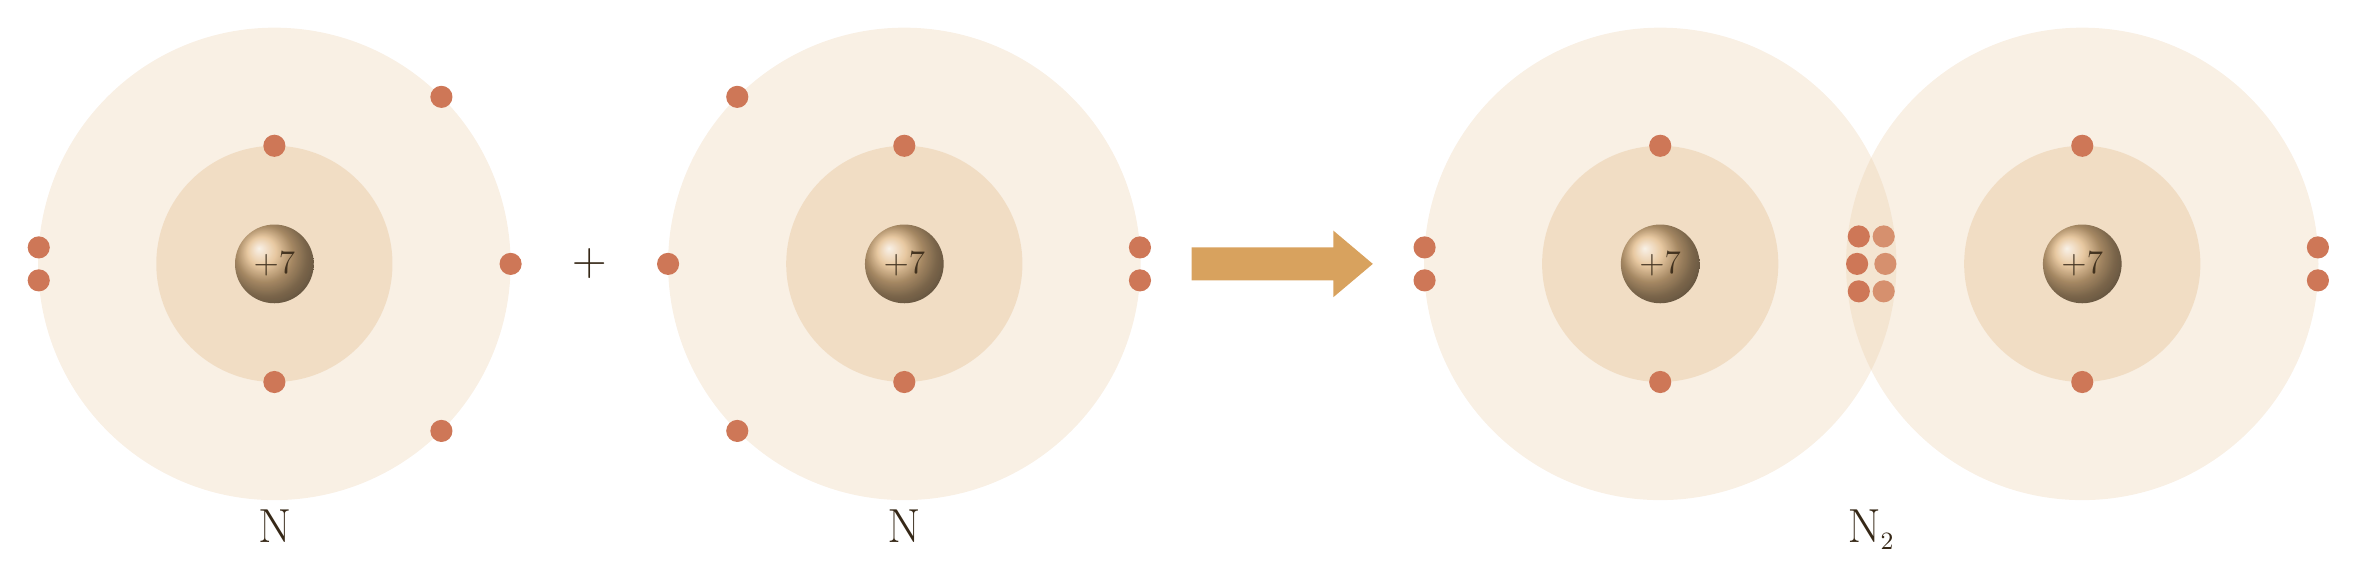
\begin{tikzpicture}[declare function={%
			r1=0.5cm;
			r2=1.5cm;
			r3=3cm;
			d=8cm;
			}
			]%
			\tikzset{
				nitrogen/.pic={
					\path[fill=\mycolor!55,opacity =0.3,pic actions] (0,0) circle (r3);
					\path[fill=\mycolor!65,opacity =0.4,pic actions] (0,0) circle (r2);
					\path[ball color=\mycolor!80,opacity =0.9,pic actions] (0,0) circle (r1) node[font=\large\fontfamily{qag}\selectfont,text=\mycolor!25!black] {$\textbf{+7}$};
					\foreach \g/\r in{90/r2,-90/r2,176/r3,184/r3}{%
						\fill (\g:\r) [\maunhan!35!\mycolor] circle (4pt);
					}
					%%
					\foreach \g/\r in{-45/r3,0/r3,45/r3}{%
						\fill (\g:\r) [\maunhan!35!\mycolor] circle (4pt);
					}
				},
				nitrogenH/.pic={
					\path[fill=\mycolor!55,opacity =0.3,pic actions] (0,0) circle (r3);
					\path[fill=\mycolor!65,opacity =0.4,pic actions] (0,0) circle (r2);
					\path[ball color=\mycolor!80,opacity =0.9,pic actions] (0,0) circle (r1) node[font=\large\fontfamily{qag}\selectfont,text=\mycolor!25!black] {$\textbf{+7}$};
					\foreach \g/\r in{90/r2,-90/r2,176/r3,184/r3}{%
						\fill (\g:\r) [\maunhan!35!\mycolor] circle (4pt);
					}
					%%
					\foreach \g/\r in{-7/r3-4pt,0/r3-4pt,7/r3-4pt}{%
						\fill (\g:\r) [\maunhan!35!\mycolor] circle (4pt);
					}
				},
				stylefont/.style={font=\bfseries\LARGE\fontfamily{qag}\selectfont,text=\mycolor!25!black}
			}
		%%%Vẽ nguyen tử thứ nhất
		\path (0,0) pic[local bounding box =na] {nitrogen};
		\path (na.south) node[anchor=north,stylefont] {N};
		%%%%vẽ dấu cộng
		\path (0.5*d,0) node[stylefont] {+};
		%%%Vẽ nguyen tử thứ hai
		\path (d,0) pic[rotate=180, local bounding box =nb] {nitrogen};
		\path (nb.south) node[anchor=north,stylefont] {N};
		\path (1.6*d,0) node {
			\tikz{
			\fill[\mycolor](0,0)--++(-90:6pt) coordinate (A)
			--++(-1.8cm,0)--++(-90:12pt)--++(0:1.8cm)coordinate (B)
			--++(-90:6pt)--($(A)!0.5!(B)+(0.5cm,0)$)--cycle;
		}
		};
		%%%Vẽ phân tử Nitrogen
		\path (2.2*d,0) pic[local bounding box =nc] {nitrogenH};
		\path (2.87*d,0) pic[rotate=180,local bounding box =nd] {nitrogenH};
		\path ($(nc.south)!0.5!(nd.south)$) node [anchor=north,stylefont] {N$_\textbf{\small2}$};
	\end{tikzpicture}
\end{document}